\section{Optimisation Problems}
An Optimisation Problem~(OP) is a problem which has a score function and bounds where the main task is to find a input that optimises the score function. Optimisation problems can be categorised as \textit{discrete optimisation problem~(DOP)} or \textit{continuous optimisation problem~(COP)} whether the variables of the problem are discrete or continuous. 
Formally speaking, an OP can be described as follows:
\begin{equation*}
min\;f(x), x \in \chi,\quad s.t.\:\Omega
\end{equation*}
where $\chi \subset\mathbb{R}^{n}$ is the search space defined over a set of \textit{n} decision variables  $x = ~(x_{1}, x_{2},..., x_{n})$, $f: \chi \rightarrow \mathbb{R}$ is the score function and $\Omega$ is the restrictions set in $x$. This is the definition for a minimisation DOP, although it would be equivalent for a maximisation DOP changing $min\;f(x)$ by $max\;f(x)$. The same happens for a COP, if in addition the decision variables are set over $\mathbb{Z}^{n}$ instead of $\mathbb{R}^{n}$ .

Furthermore, optimisation problems may have more than one score function and they are called \textit{Multi-Objective Optimisation Problems~(MOOP)}. This is the primary field of study in this work so, hereinafter all the references to optimisation problems in this work will be to MOOP.
\newpage
\subsection{Multi-Objective Optimisation Problems}

Multi-Objective Optimisation Problems~(MOOPs) are optimisation problems which have two or more objective functions to optimise and those objective functions can take opposite directions (thinking about directions as \textit{minimise or maximise}). Besides, a MOOP can discrete or continuous considering whether the variables of the problem are discrete or continuous. \\
Formally speaking, a MOOP can be described as finding a vector \textbf{$x$} inside the problem's search space \textit{$\chi$} in such way that optimises the vector of objective functions \textit{$f(x)$}\cite{search}:
\begin{align*}
min\;f(x) & = (f_{1}(x), f_{2}(x), ..., f_{k}(x)), \: x\;\in\chi \\
 g_{i}(x) & \leq 0, \: i = 1, 2, ..., q. \\
 h_{i}(x) & \leq 0, \: i = 1, 2, ..., p.
\end{align*}
where $x = (x_{1}, x_{2}, ..., x_{n}) \in \mathbb{Z}^{n}$, are the objective functions to optimise $f_{i}: \mathbb{Z}^{n} \rightarrow \mathbb{R}, \; i = 1, ..., k$ being \textit{n} the number of decision variables and $g_{i}: \mathbb{Z}^{n} \rightarrow \mathbb{R}, \; i = ~1, ..., q$ and $h_{i}: \mathbb{Z}^{n} \rightarrow \mathbb{R}, \; i = 1, ..., p$ are the problem's restriction functions.

Moreover, the standard method for solving a MOOP is the well-known \textit{Pareto method}\cite{search}. The Pareto method is based on the non-dominance principle\cite{search, metaheuristics}. On the one hand, dominance means that given two solutions for a MOOP, one solutions dominates the other one when it has as least the same quality for every objective and, it has strictly more quality for one of them than the other solution. Formally, this can be expressed as follows\cite{search}:
\begin{align*}
A \succeq  B \Leftrightarrow & \forall i \in \{1, 2, ..., n\} \: a_{i} \leq b_{i}, \\
& y\;\exists i \in \{1, 2, ..., n\}, \: a_{i} < b_{i}
\end{align*}

On the other hand, it is the direction conflict between objectives which leads to solutions with trade-offs between those objectives. So, at this point it is where the \textit{non-dominance} appears. The non-dominance refers the situation where a solution it is not dominated by any other solution of the problem. That means that it can not be found any other solution to the problem which increases the quality of any objective without irredeemably decreases the quality of another one. Non-dominated solutions may be found at the limits of the search space (\textit{$\chi$}) and are those which shape the Pareto set.
%%%%%%%%%%%%%%%%%%%%%%%%%%%%%%%%%%%%%%%%%%%%%%%%%%%%%%%%%%%%%%%%%%%%%%%%%%%%%%%%%%%%
\newpage
\section{Evolutionary Algorithms}

Nowadays, there are many methods for solving MOOPs but they can be classified merely in two types of methods: \textit{approximated methods and exacts methods}. The different categories of exact and approximated methods can be seen down below.

\begin{figure}[!h]\label{opt_met}
\centering
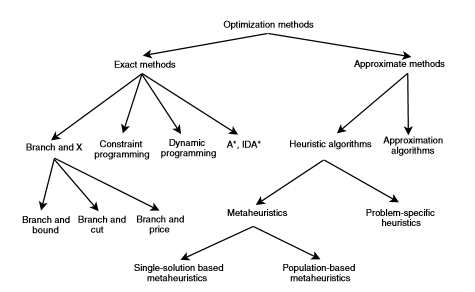
\includegraphics[width=0.8\textwidth]{mem/images/meta.png}
\caption{Optimisation methods}
\end{figure}

On the one hand, \textit{exacts methods} are those which ensure that, if there is an optimal solution to the facing problem they will be able to find it. However, these methods that guarantees reaching the optimal solution, they have a important drawback, its performance. Assuring the optimal solution implies increasing the computational work and hence more time to obtain the solution.

On the other hand, \textit{approximated methods} are very popular nowadays even though they do not guarantee reaching the optimal solution for a problem. Nevertheless, approximated methods can obtain high quality solutions in an assumable time due they set a balance between computational performance and solution quality. 

Approximated methods can be divided in two categories: \textit{heuristic algorithms} and \textit{metaheuristics algorithms}. However, this work it is focus primarily in \textit{metaheuristics algorithm} and even more specifically in the field of \textit{evolutionary algorithms}.

Evolutionary algorithms~(EA) develop the metaphor of natural evolution, the survival of the fittest individual\cite{eiben}. This is, given a population of individuals in some environment with limited resources, the competition for surviving causes natural selection and the fittest individuals are more likely to survive and reproduce. Nevertheless, there are several variants of EA and they can be classified as:
\begin{enumerate}
    \item Genetic Algorithms\cite{Whitley1994, Algorithms2004, Sivanandam2008}.
    \item Evolutionary Strategies\cite{Beyer2002, Hansen2017}.
    \item Differential Evolution\cite{Algorithm2006, DE1, DE2, DE3}.
\end{enumerate}

Considering the field of optimisation problems, the natural evolution metaphor is develop as follows:
\begin{enumerate}
    \item The problem to solve and its bounds is the environment with limited resources.
    \item A set of random initial solutions for the given problem are the first individuals at generation zero. 
    \item The population of individuals reproduce between each other applying genetic operators to generate offspring. Commonly combination and mutation.
    \item At each generation, the individuals within a population compete and the fittest individuals (the better quality solutions) survive.
    \item Steps three and four are repeated until reaching the stop condition.
\end{enumerate}
Generally, the before metaphor can be shown as a pseudo-code\cite{eiben}:

\begin{algorithm}[!h]
  INITIALISE population with random candidate solutions\;
  EVALUATE each candidate\;
  \While{not StopCriteria satisfied}{
    SELECT parents\;
    RECOMBINE pairs of parents\;
    MUTATE the result offspring\;
    EVALUATE new candidates\;
    SELECT individuals for the next generation\; 
  }
  \caption{General scheme of an EA.}
\end{algorithm}

%%%%%%%%%%%%%%%%%%%%%%%%%%%%%%%%%%%%%%%%%%%%%%%%%%%%%%%%%%%%%%%%%%%%%%%%%%%%%%%%%%%%%%%
\newpage
\section{Menu Planning Problem}

The Menu Planning Problem \textit{(MPP)} is a well-known NP-Problem which has been trying to computerise since 1960\cite{Ngo2016}. In essence, the MPP is to find a set of dishes combination which satisfies some restrictions of budge, variety and nutritional requirements for a \textit{n} days sequence. In addition, it can include other constraints such as user preferences, cooking time or the number for meals each day.
Traditionally, the MPP's main objective is to minimise the total cost of the meals for each day\cite{Ngo2016, Moreira2018} but it also supports other objective functions like maximising the variability or minimising the cooking time.

Furthermore, the MPP can be studied as a multi-objective problem\cite{Seljak2009, Moreira2018} if the amounts of nutrients requirements and cost of the meals are considered independent objectives. This approach leads to reduce the MPP to a Multi-dimensional Knapsack Problem \textit{(MDKP)} where the maximum amount of each nutrient define the limit of the multiple dimensions. However, the MPP is also studying as a single-objective problem where mainly research define the objective function as the total cost of the meals. For instance, a single-objective approach for the MPP is in\cite{Moreira2018} where the authors proposed an evolutionary approach to solving the 5-day Single-Objective Menu Planning Problem composed by three meals daily, using as a function to minimise the total cost of the designed menus. In addition, the set of constraints that the researchers defined to this problem are moderately different from the usual constraints set for the typical MPP. In this occasion, the authors set the student age group, the school category, school duration time, school location, variety of preparations, the maximum amount to be paid for each meal and finally, the lower and upper limits of macro-nutrients as the constraints set to be satisfied for each solution to be considered feasible. Within this research, the authors used the generic Genetic Algorithm (GA) for the computational experiments. The results obtained from the generic GA where compared with a Greedy-based approach. The results prove that the GA outperforms the Greedy-based approach when the limit values of the meals are fixed at R\$ 2.00 for breakfast, R\$ 4.00 for lunch and R\$ 2.00 for the snack. (BRL - R\$ 1.0 ~~ USD - \$ 0.31).

In the other hand, in the paper\cite{Funabiki2011}, the authors refer to the Two-phase Cooking N-day Menu Planning Problem where the objective is to maximise the preferences among the selected foods in the menu plan. The conditions which shape the set of constraints that must be satisfied are only three. The total cooking time of any day must not exceed the limit specified, only foods that which allow two-phase cooking can be selected for two-phase cooking and finally, the food cannot be repeated more times than a certain repeat constraint. In order to face this problem, the researchers used a simple greedy method prioritising the user-specified preference with the cooking time of each food.

Eventually, another study where the MPP is faced as a single-objective problem is\cite{Sufahani2014}. Here, the authors set up a mathematical model to solve the MPP considering only one objective function. The model's goal is to minimise the budget provided by the government subject to the restriction of trying to maximise the variety of dishes. Furthermore, the model tries to create menus in such a way they maximise the nutritional requirements. For the computational experiments, the researchers programmed an Integer Programming algorithm in Matlab using LPSolve. Furthermore, the given results, taking into account that the optimal solution was found within one second, are better compared to other heuristics like GA.

\textcolor{red}{As can be seen, there is a certain variety within the optimisation methods for solving the single-objective MPP approach. Despite that, Evolutionary Computing \textit{(EC)} techniques, such as GA, are mostly cited in the related bibliography as a good choice\cite{Ngo2016, Seljak2009, Moreira2018}}. 

\textcolor{red}{Nevertheless, there is not any study which compares the performance and results between the multi-objective MPP and the single-objective MPP.}